% -*- TeX:Rnw -*-
% ----------------------------------------------------------------
% .R Sweave file  ************************************************
% ----------------------------------------------------------------
%%
%\documentclass[a4paper,12pt,english]{article}
\documentclass[a4paper,12pt,slovene]{article}
\usepackage{babel}
\newcommand{\naslov}{Stat 07-08}
\input{abpkg}
\input{abcmd}
\input{abpage}

\usepackage{pgf,pgfarrows,pgfnodes,pgfautomata,pgfheaps,pgfshade}
\usepackage{amsmath,amssymb}
\usepackage{colortbl}
\usepackage{Sweave}
\input{mysweave}
\usepackage{lmodern}
\input{abfont}
%\SweaveOpts{keep.source=true}
%\setkeys{Gin}{width=0.8\textwidth} % set graphicx parameter
% ----------------------------------------------------------------
\begin{document}
%% Sweave settings for includegraphics default plot size (Sweave default is 0.8)
%% notice this must be after begin{document}
%%% \setkeys{Gin}{width=0.9\textwidth}
% ----------------------------------------------------------------
\title{Analiza podatkov Statistika 2007/08}
\author{A. Blejec}
%\address{}%
%\email{}%
%
%\thanks{}%
%\subjclass{}%
%\keywords{}%

%\date{}%
%\dedicatory{}%
%\commby{}%
\maketitle
% ----------------------------------------------------------------
\begin{abstract}
Analiza podatkov in kak�na re� za predavanja in vaje
\end{abstract}
% ----------------------------------------------------------------

\section{Priprava podatkov}

\begin{Schunk}
\begin{Sinput}
> data <- read.xls("../data/podatki0708.xls")
> summary(data[, -1])
\end{Sinput}
\begin{Soutput}
    skupina         starost         rojenec      spol        teza       
 Min.   :1.000   Min.   :19.00   Min.   :1.000   F:53   Min.   : 45.00  
 1st Qu.:2.000   1st Qu.:20.00   1st Qu.:1.000   M: 8   1st Qu.: 59.00  
 Median :2.000   Median :20.00   Median :1.000          Median : 64.00  
 Mean   :2.443   Mean   :20.30   Mean   :1.475          Mean   : 64.21  
 3rd Qu.:3.000   3rd Qu.:20.00   3rd Qu.:2.000          3rd Qu.: 69.00  
 Max.   :4.000   Max.   :22.00   Max.   :3.000          Max.   :105.00  
                                                                        
     visina          razpon       cevelj         lasje        
 Min.   :155.0   Min.   :152.0   Mode:logical   Mode:logical  
 1st Qu.:165.0   1st Qu.:164.0   NA's:61        NA's:61       
 Median :171.0   Median :170.5                                
 Mean   :170.7   Mean   :170.9                                
 3rd Qu.:176.0   3rd Qu.:176.0                                
 Max.   :191.0   Max.   :191.0                                
                 NA's   :  1.0                                
   oci          ociMati         ociOce         klicna       
 Mode:logical   Mode:logical   Mode:logical   Mode:logical  
 NA's:61        NA's:61        NA's:61        NA's:61       
\end{Soutput}
\begin{Sinput}
> data <- data[data$spol == "F", ]
> attach(data)
> n <- length(id)
\end{Sinput}
\end{Schunk}

\begin{Schunk}
\begin{Sinput}
> par(mfrow = c(2, 2))
> xlim <- range(c(visina, razpon), na.rm = TRUE) * c(0.95, 
+     1.05)
> barplot(table(starost), col = "lightblue", main = "starost")
> hist(visina, col = "lightblue", xlim = xlim)
> rug(jitter(visina))
> hist(teza, col = "lightblue")
> rug(jitter(teza))
> hist(razpon, col = "lightblue", xlim = xlim)
> rug(jitter(razpon))
\end{Sinput}
\end{Schunk}
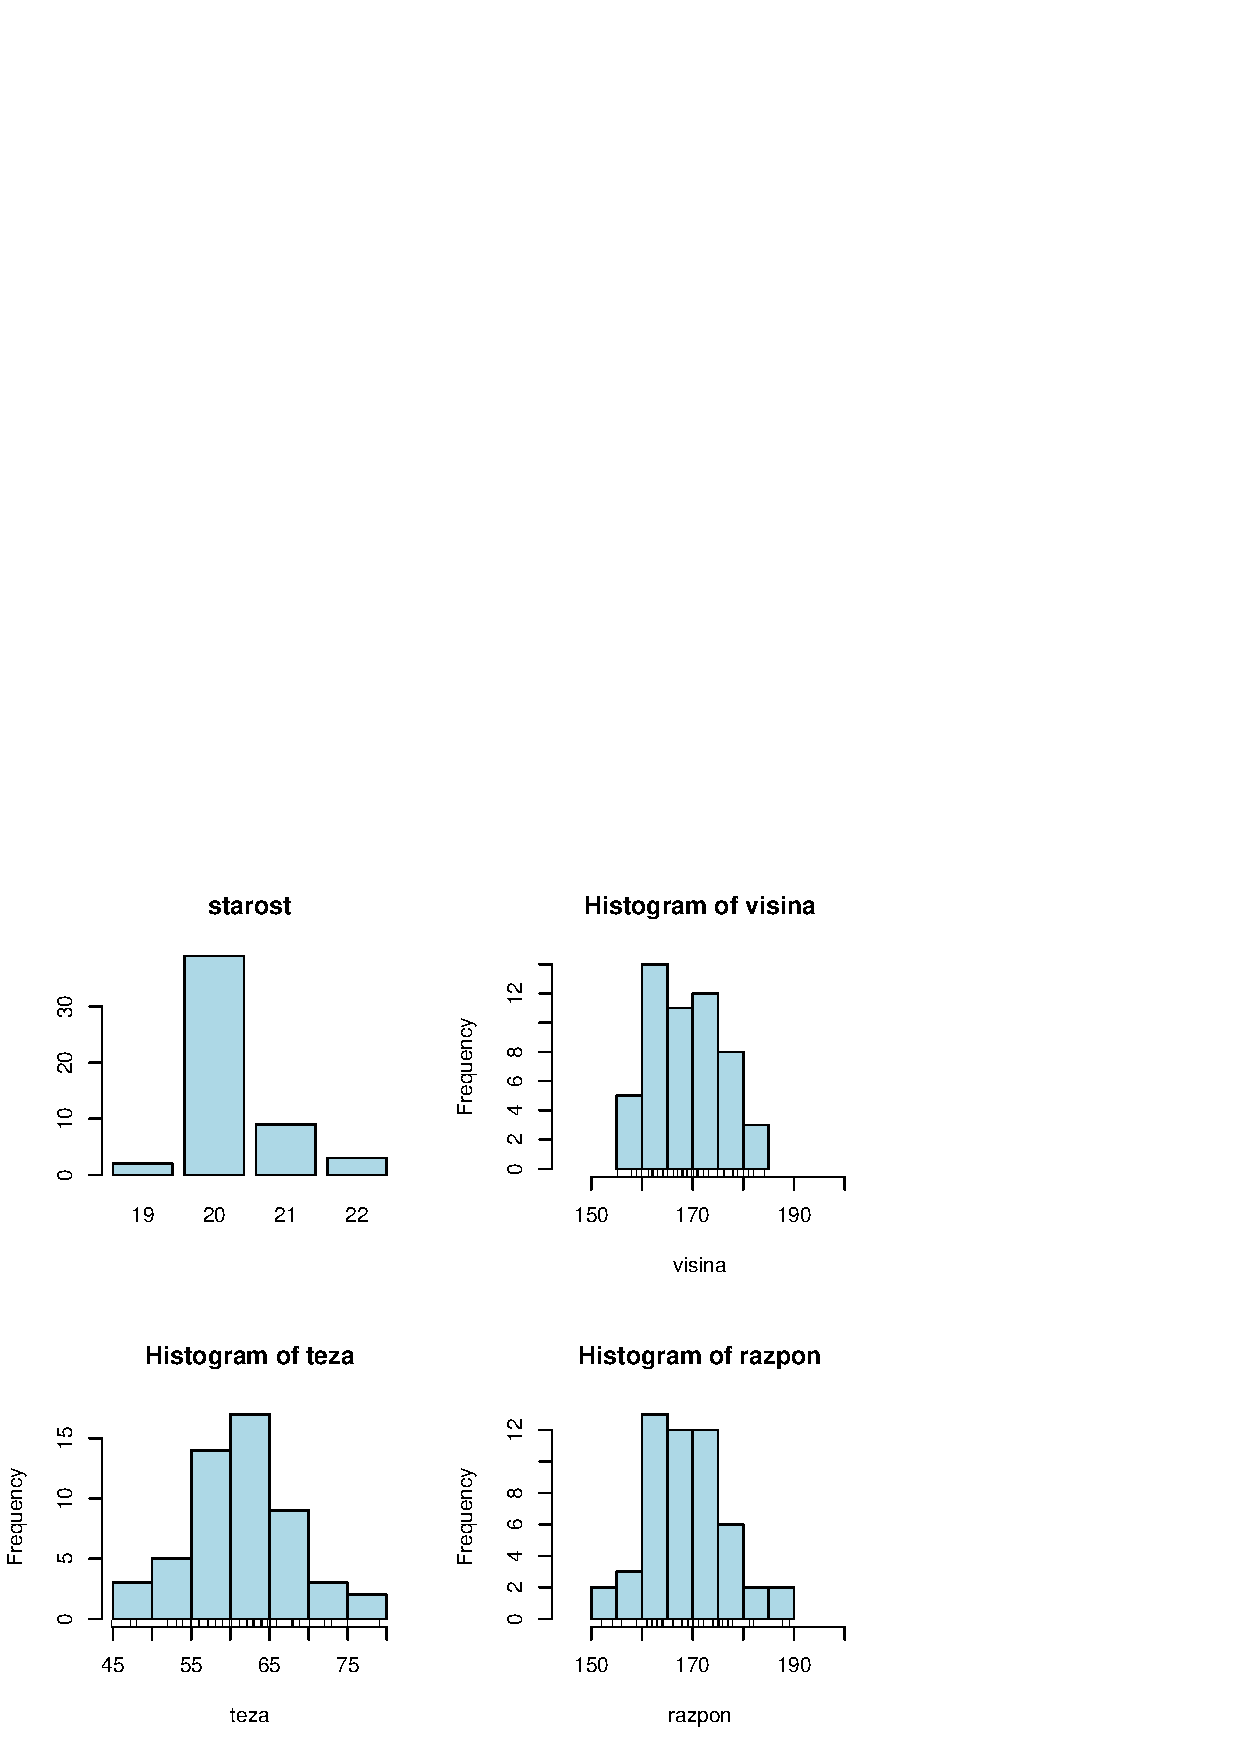
\includegraphics{Opisna-003}

\begin{Schunk}
\begin{Sinput}
> plot(sort(visina), 1:n)
> points(sort(visina), 1:n)
> v <- order(visina)
> lines(visina[v], rank(visina)[v], pch = 16, col = "red", 
+     type = "o", cex = 1.2)
> table(visina)
\end{Sinput}
\begin{Soutput}
visina
155 158 159 160 161 162 163 164 165 166 167 168 169 170 171 172 173 175 
  1   1   1   2   1   3   3   3   4   1   3   3   2   2   5   4   2   1 
176 178 179 180 181 182 184 
  3   2   1   2   1   1   1 
\end{Soutput}
\begin{Sinput}
> lines(as.numeric(names(table(visina))), table(visina), type = "h", 
+     lwd = 3)
> boxplot(visina, horiz = TRUE, add = TRUE)
\end{Sinput}
\end{Schunk}
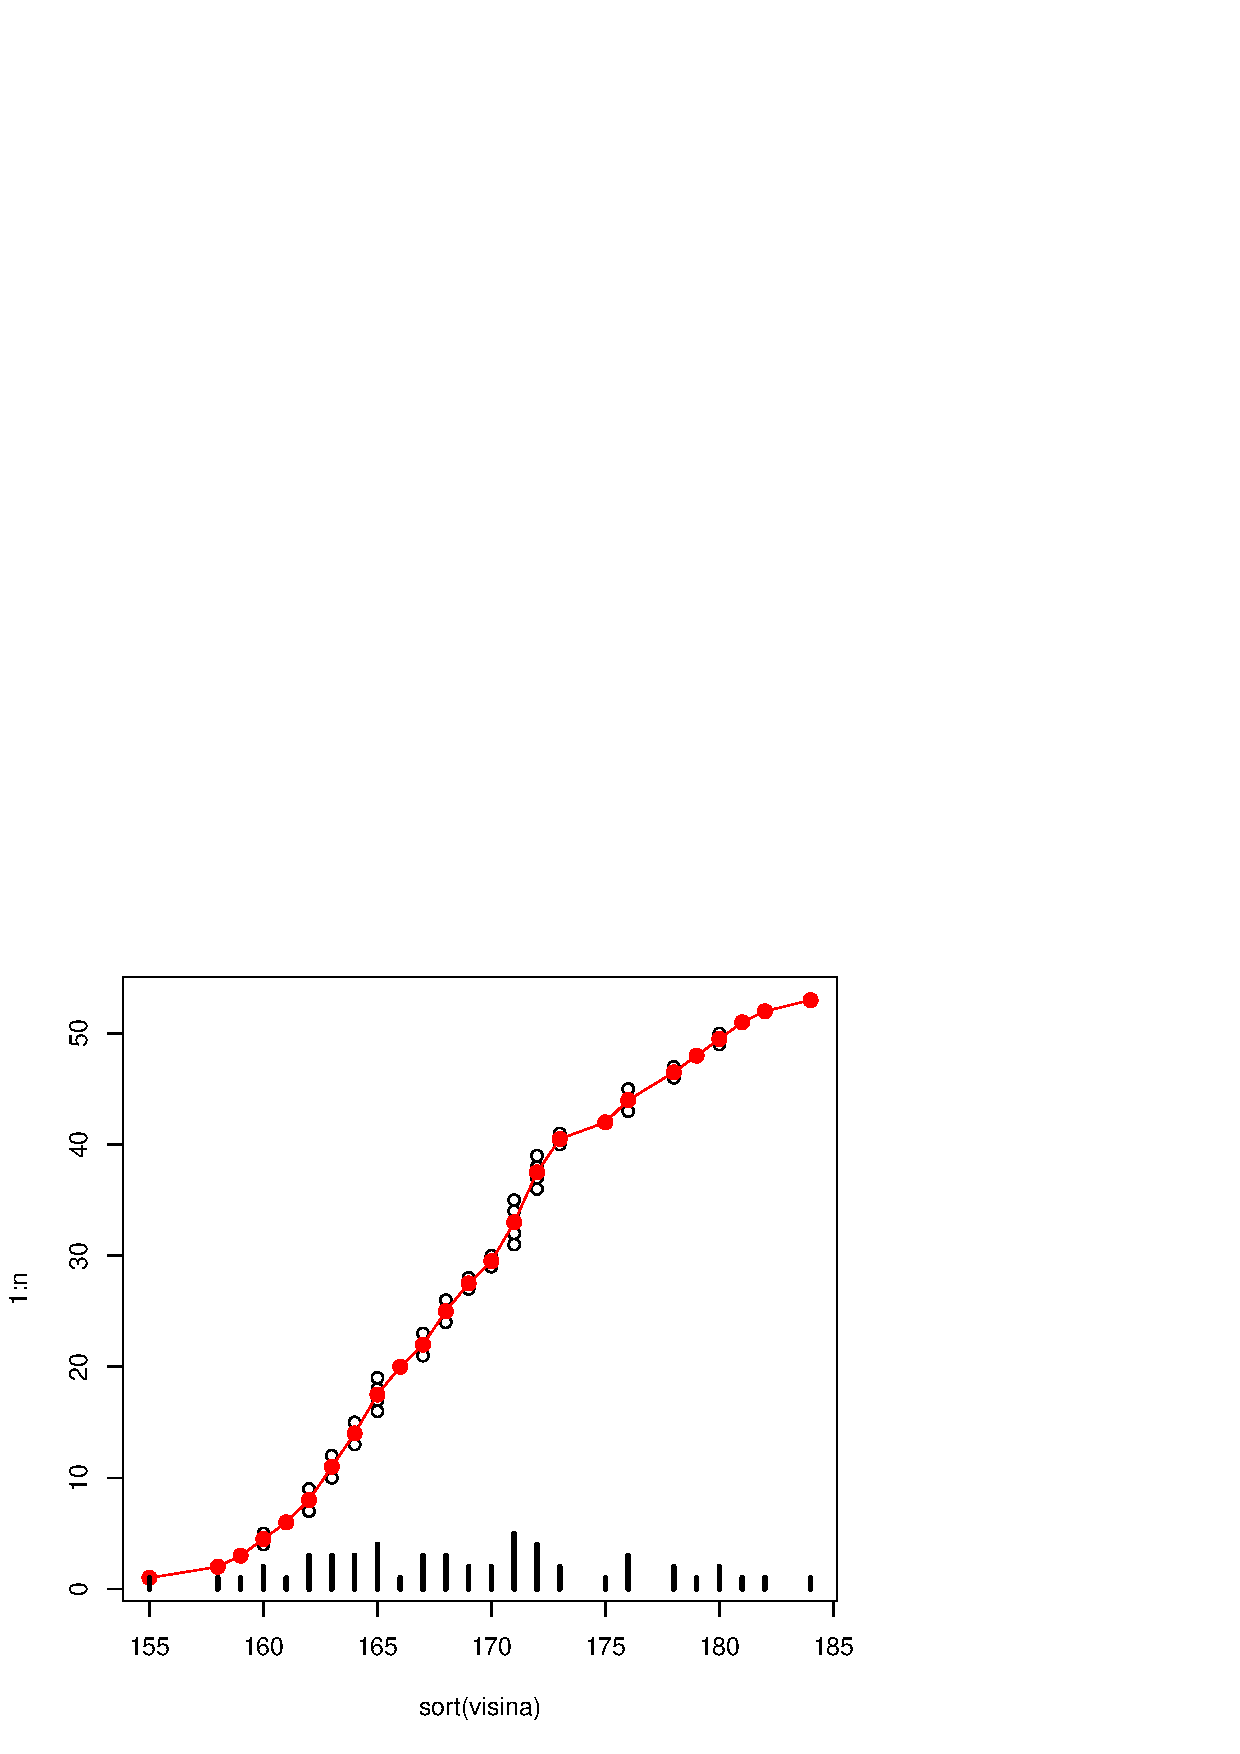
\includegraphics{Opisna-005}



% ----------------------------------------------------------------
%\bibliographystyle{amsplain}
%\bibliography{}
\end{document}
% ----------------------------------------------------------------
